\section{Partitionnement automatique}Pendant le partitionnement automatique, toutes les donn\'ees sur le disque dur seront effac\'ees et deux partitions nouvelles seront \'etablies. Il seraient \'etablies une partition pour les donn\'ees et le syst\`eme d'exploitation et une autre partition pour la permutation.\\
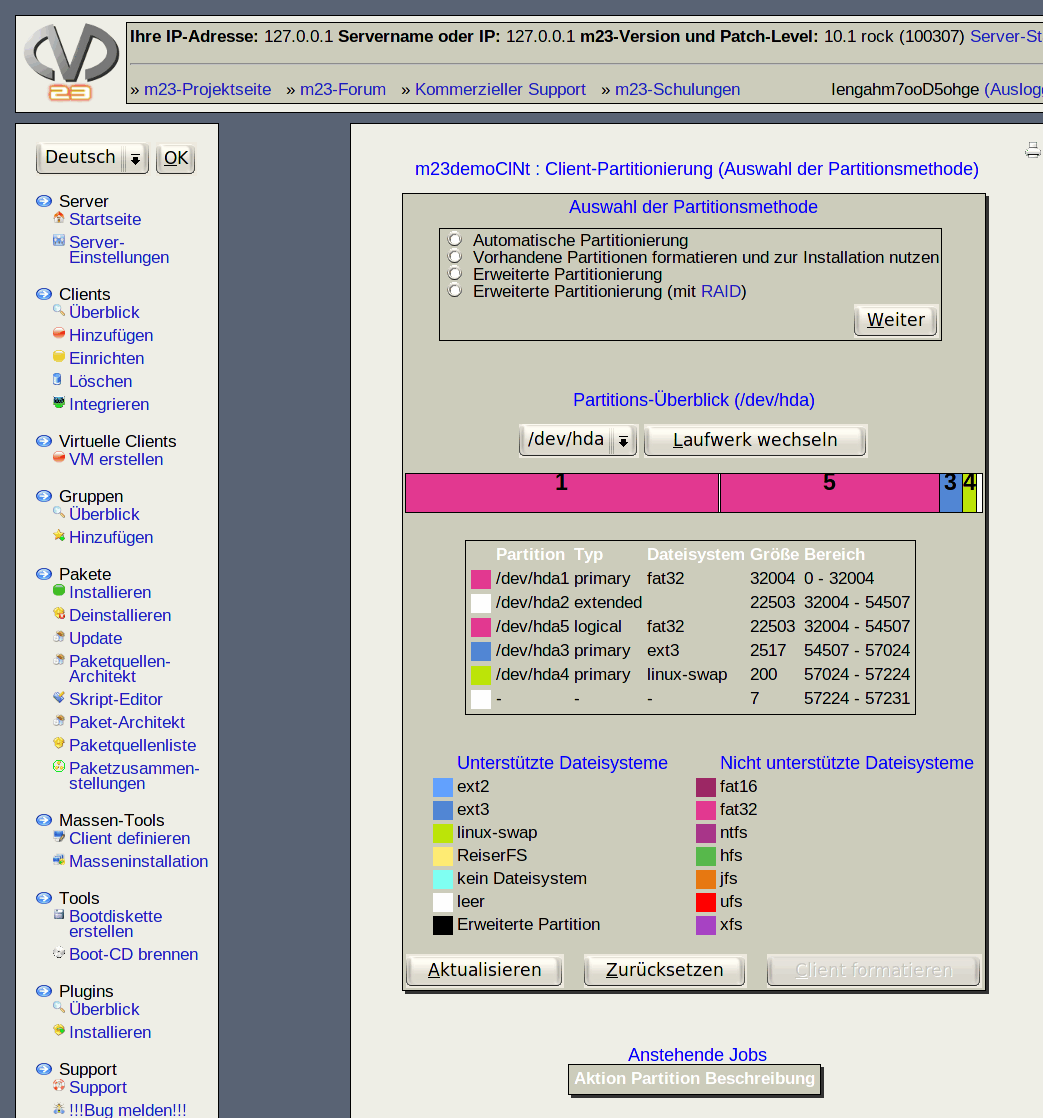
\includegraphics[scale=0.4]{/mdk/doc/manual/screenshots/fr/fdisk-automatic.png} \\
\subsection{Proc\'ed\'e \'etape par \'etape:}
\begin{enumerate}
\item Choisissez \textit{$\ll$Partitionnement automatique$\gg$}.\\
\item Apr\`es avoir cliqu\'e sur \textit{$\ll$Actualiser$\gg$}, vous pourriez voir le partitionnement sugg\'er\'e.\\
\item Acceptez les suggestions en cliquant sur \textit{$\ll$Formater le poste client$\gg$}.\\
\end{enumerate}
